\chapter{Fluid-Structure Interaction}\label{chap:fsi}
\section{Introduction}
In the current chapter, we couple the CTVF scheme developed in \cref{chap:ctvf}
to model fluid-structure interaction problems. Fluid-structure interaction (FSI)
is a common engineering problem that is seen in daily life. Some examples
include the deformation of wind turbine blade due to the fluid flow, blood flow
in heart value, coastal engineering, and vortex-induced vibration
\citep{williamson2004vortex,bearman2011circular}. An accurate study of FSI can
allow us to optimize the systems where FSI is dominant. However, studying the
FSI phenomena through experiments or analytical techniques are complex due to
their nonlinear behavior.

Handling FSI problems with the transport velocity formulation framework is
advantageous as it can solve the tensile instability issue in solid dynamics and
ensure a homogeneous particle distribution in fluids. In the current chapter, we handle
FSI problems by the CTVF method, where both fluids and solid phases are modeled
using CTVF alone. To validate the proposed method, we consider three numerical
test cases. A uniformly distributed load over a clamped beam (UDL) problem is
considered to validate the elastic dynamics of CTVF. An aluminum plate over a
hydrostatic tank for FSI validation is considered. Finally, it is applied to a
fluid flow striking an elastic plate. Here, the deformation of the elastic plate
is compared against the experimental results.

\section{Numerical Modeling}\label{sec2}
We follow the CTVF formulation to model both fluid and solid phases. The
particles are moved with a transport velocity rather than the momentum velocity,
which provides us with a homogenized particle distribution and eliminates
tensile instability. In the following two sections we briefly describe the
governing equations of the fluid and solid dynamics in discretized form.


\subsection{Discrete Equations of the Fluid and Solid Medium}\label{subsec:discrete-fluid}
The governing equations of the fluid are conservation of mass and momentum. We
follow the SPH discretization of the continuity
equation~\eqref{eq:fsi:sph-discretization-continuity} and the EDAC
based~\citep{PRKP:edac-sph-iccm2015} pressure evolution
equation~\eqref{eq:fsi:sph-discretization-edac} given in \cref{chap:ctvf}, given
as
\begin{equation}
  \label{eq:fsi:sph-discretization-continuity}
  \frac{\tilde{d}\rho_a}{dt} = \sum_{b} \; \frac{m_b}{\rho_{b}} \; (
  \rho_{a} \; \tilde{\ten{u}}_{ab} \; + \;
  (\rho \; (\tilde{\ten{u}} \; - \;
  \ten{u}))_{ab}) \; \cdot \nabla_{a} W_{ab},
\end{equation}
\begin{multline}
  \label{eq:fsi:sph-discretization-edac}
  \frac{\tilde{d}p_a}{dt} = \sum_{b} \; \frac{m_b}{\rho_{b}} \; \bigg(
  (p_{a} - \rho_{a} c_{s}^2) \; \ten{u}_{ab} \; + \;
  p_{a} \; \tilde{\ten{u}}_{ab} \; - \;
  (p \; (\tilde{\ten{u}} - \ten{u}))_{ab} \; + \;
  4 \; \nu_{edac}
  \frac{p_a - p_b}{(\rho_a + \rho_b) (r^2_{ab} + 0.01 h_{ab}^{2})} \ten{r}_{ab}
  \bigg) \; \cdot \nabla_{a} W_{ab}.
\end{multline}
%
Here, the summation also includes the solid particles in the influence of a
fluid particle. The momentum equation is modified to consider the force
acting on the fluid particle due to the interaction with the elastic structure
particles. The discretized momentum equation is written as,
\begin{multline}
  \label{eq:fsi:sph-momentum-fluid}
  \frac{\tilde{d}\ten{u}_{a}}{dt} = - \sum_{b} m_b \bigg[
  \bigg(\frac{p_a}{\rho_a^2} + \frac{p_b}{\rho_b^2}\bigg) \ten{I} -
  \bigg(\frac{\ten{A}_a}{\rho_a^2} + \frac{\ten{A}_b}{\rho_b^2} + \Pi_{ab}
  \ten{I} \bigg) \bigg]
  \cdot \nabla_{a} W_{ab} \\
  + \ten{u}_{a} \sum_{b} \frac{m_b}{\rho_{b}} \; \tilde{\ten{u}}_{ab} \cdot
  \nabla_{a} W_{ab} \\+ \sum_{b} m_b \frac{4 \eta \nabla W_{ab}\cdot
    \ten{r}_{ab}}{(\rho_a + \rho_b) (r_{ab}^2 + 0.01 h_{ab}^2)} \ten{u}_{ab} +
  \ten{g}_{a} + \frac{\ten{F}^a_{\text{FSI}}}{m_a}
\end{multline}
$\ten{F}^a_{\text{FSI}}$ is the force due to the interaction with elastic
structure. This force modeling is explained in \cref{subsec:fsi}. We utilize the
ghost particle approach proposed in \citep{Adami2012} to handle the boundaries.


Similar to the governing equations for the fluid, the governing equations of
the solid phase follow \cref{chap:ctvf} with a modification to the momentum
equation. We additionally need to consider the force due to the
fluid particles. The resulting equation is given as
\begin{multline}
  \label{eq:fsi:sph-momentum-solid}
  \frac{\tilde{d}\ten{u}_{a}}{dt} = - \sum_{b} m_b \bigg[
  \bigg(\frac{p_a}{\rho_a^2} + \frac{p_b}{\rho_b^2}\bigg) \ten{I} -
  \bigg(\frac{\teng{\sigma}^{'}_{a}}{\rho_a^2} +
  \frac{\teng{\sigma}^{'}_{b}}{\rho_b^2} + \Pi_{ab} \ten{I} \bigg) \bigg]  \cdot \nabla_{a} W_{ab}
  + \ten{g}_{a} + \frac{\ten{F}^a_{\text{FSI}}}{m_a}.
\end{multline}

We utilize SPST formulation described in \cref{sec:sunpst} to compute the
transport velocity of the fluid particles, while for the elastic phase
IPST \citep{huang_kernel_2019} formulation is used.

\subsection{Fluid-Structure Interaction}\label{subsec:fsi}
Coupling is handled in a straight forward way in SPH. While modelling the fluid
phase and treating the fluid-structure interactions, the solid particles are
assumed to be boundary particles. From the boundary handling given in Adami
\citep{Adami2012}, we compute the pressure of the boundary particles from
the extrapolated equation as,
\begin{equation}
  \label{eq:fsi:pressure-bc}
  p_s = \frac{\Sigma_f p_f W_{sf} + (\ten{g} - \ten{a}_{\ten{s}}) \cdot \Sigma_f
    \rho_f \ten{r}_{sf} W_{sf}}{\Sigma_f W_{sf}}.
\end{equation}
Here, $\ten{a}_s$ is the acceleration of the structure particles. The subscript
$f$ denotes the fluid particles and $s$ denotes the solid particles. Using the
extrapolated pressure, the hydrodynamic density of solid particles are
computed. Please note that the pressure we set here only pertain to the
FSI force and does not correspond to the real pressure or density of the
solid particles. By utilizing the previously set hydrodynamic properties on
the structure, the interaction force is computed using,
\begin{equation}
  \ten{F}_{\text{FSI}}^f = -m_f \sum_{s} m_s \bigg(\frac{p_f}{\rho_{f}^2} +
  \frac{p_s}{\rho_{s}^2} + \Pi_{fs} \bigg) \nabla_{f} W(x_{fs}).
\end{equation}


\section{Results And Discussion}\label{sec3}
In the current section we simulate three numerical examples to validate the
developed model. Deformation of a UDL plate due to external force and
hydrodynamics loads from a hydrostatic tank. Further, the model is applied to
study the deformation of an elastic obstacle due to the impact of fluid. A
convergence study is undertaken for both the UDL and elastic deformation under
hydrodynamic load problems. All the results are fully automated with the automan
package \citep{automan2018} and made easy to reproduce. The source code for all
the problems demonstrated in this manuscript is made available at
\url{https://github.com/dineshadepu/fsi_etvf}.

% =========================================
% =========================================
% start
% =========================================
% =========================================
\subsection{Uniformly Distributed Loading (UDL) on a Clamped Beam}
\label{sec:udl}
In the first test case, we validate the structural part of the current solver.
We consider a homogeneous elastic plate clamped on both ends acted upon by a
uniformly distributed load ($q = 20$ Nm$\textsuperscript{-1}$) as shown in
\cref{fig:udl-schematic}. The beam's length (L) and height (H) is 0.2 m and
\begin{figure}
  \centering
  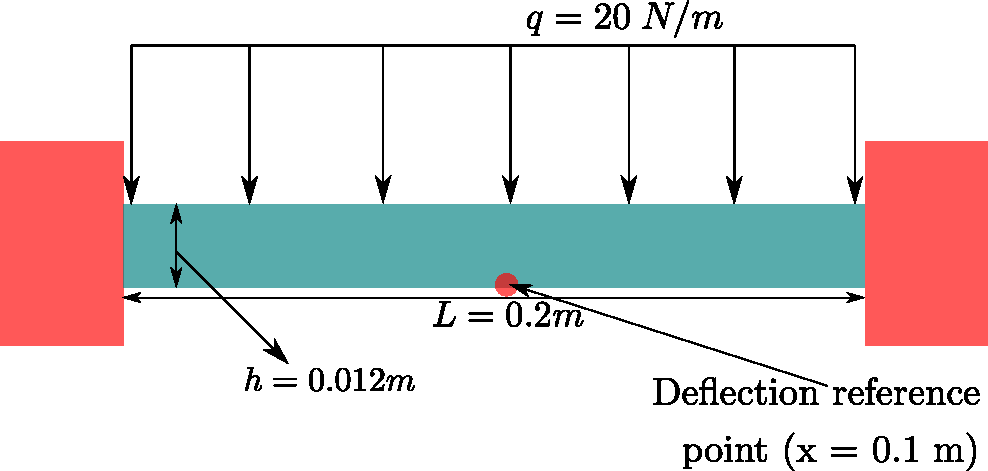
\includegraphics[scale=0.5]{images/fsi/images/khayyer_2021_udl/schematic}
  \caption{The schematic of a clamped elastic beam being acted upon by a
    uniformly distributed load.}
\label{fig:udl-schematic}
\end{figure}
$0.012$ m, respectively. The mechanical properties of the plate are set as
$E=10^7$ Pa in Young's modulus, $\nu=0$ in Poisson's ratio and $\rho=1000$
kgm$\textsuperscript{-3}$ in density. The numerical solution of the
y-displacement at the center of the beam is compared against the analytical
counterpart. The analytical solution for the deflection of a uniformly
distributed beam clamped at both ends is given by
\begin{equation}
  \label{eq:fsi:ce-tvf}
  \eta\left(\frac{L}{2}\right) = \frac{qL^4}{384 D},
\end{equation}
where, $D$ is defined as $\frac{E h^3}{12 (1 - (\nu)^2)}$. We consider three
particle resolutions such that, $10$, $15$, and $20$ particles along the beam's
width are used. We run for a total physical time of $2$ seconds.

\Cref{fig:udl-disp-plot} depicts the time history of y-displacement of the beam
center for different particle resolutions computed using the current solver
compared against the analytical solution. From \cref{fig:udl-disp-plot}, we can
see that the current solver can accurately predict the displacement of the
\begin{figure}
  \centering
  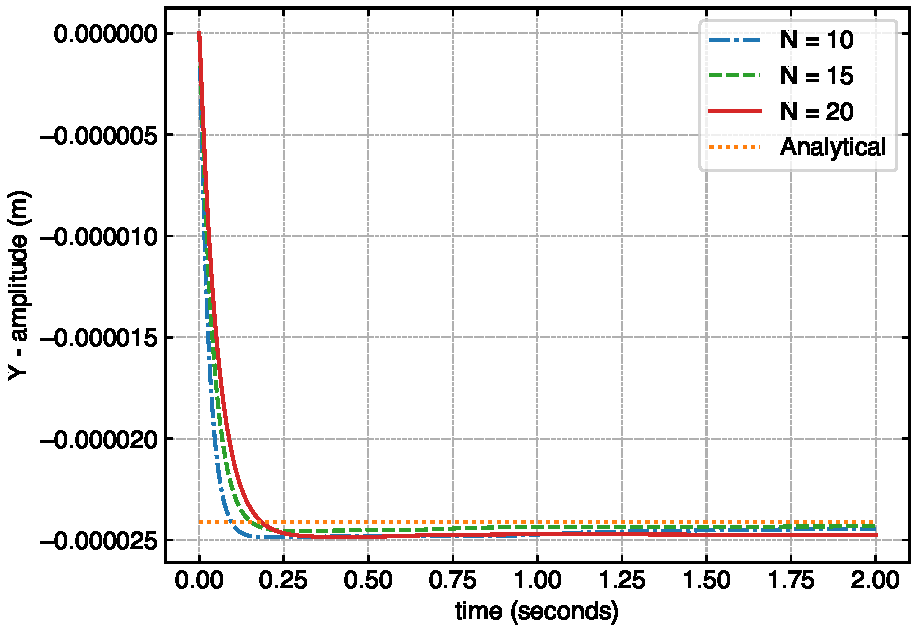
\includegraphics[scale=0.5]{figures/fsi/figures/khayyer_2021_udl/homogenous}
  \caption{Time variation of the y-displacement of the center of the beam for
    three different resolutions, compared against the analytical result.}
\label{fig:udl-disp-plot}
\end{figure}
clamped beam. Convergence of the current scheme is captured in
\cref{fig:udl-disp-plot}, and the computational results are within a reasonable
variation of the analytical solution with the variation of the particle spacing.


\subsection{Hydrostatic Water Column on an Elastic Plate}
\label{sec:hydrostatic-water-column-on-an-composite-elastic-plate}
In this example, we study the deformation of an elastic plate due to the
hydrostatic water column. We utilize the current example to examine the accuracy
and convergence of the current solver. The schematic of fluid with the elastic
beam is shown in \cref{fig:hs-water-on-plate} along with the initial pressure
distribution in the fluid. The figure includes the dimensions as well. The
material properties of the beam are, a density of $2700$
kgm\textsuperscript{-3}, with an Young's modulus of $67.5$ GPa, and a Poisson
\begin{figure}
  \centering
  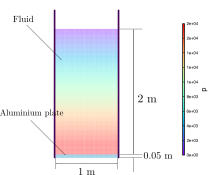
\includegraphics[scale=0.4]{images/fsi/images/ng_2020_hydrostatic_water_column_on_elastic_plate/schematic}
  \caption{Schematic of the hydrostatic water column on an elastic plate. Fluid
    particle color represents pressure.}
\label{fig:hs-water-on-plate}
\end{figure}
ratio of $0.34$. The material properties of the fluid are, a density of $1000$
kgm\textsuperscript{-3}, with a zero dynamic viscosity. We consider three particle
resolutions such that we get $10$, $15$ and $20$ particles along the width
direction of the beam. We run the simulation for a total physical time of $3$
seconds. The y-displacement of the current solver at the center of the beam is
compared against the analytical result. The beam deflection computed using
an analytical expression results in a deflection $d = -6.85 \times 10^{-5}$ m.

\Cref{fig:snapshot-hs-fsi} shows the particle plot of the fluid along with the
elastic solid at time $2$ seconds with color of the fluid particles describing
the pressure. This snapshot corresponds to the highest particle resolution i.e.,
$20$ particles along the width direction. From the \cref{fig:snapshot-hs-fsi},
we can see that the current solver produces a smooth pressure distribution
\begin{figure}[!htpb]
  \centering
  \begin{subfigure}{0.48\textwidth}
    \centering
    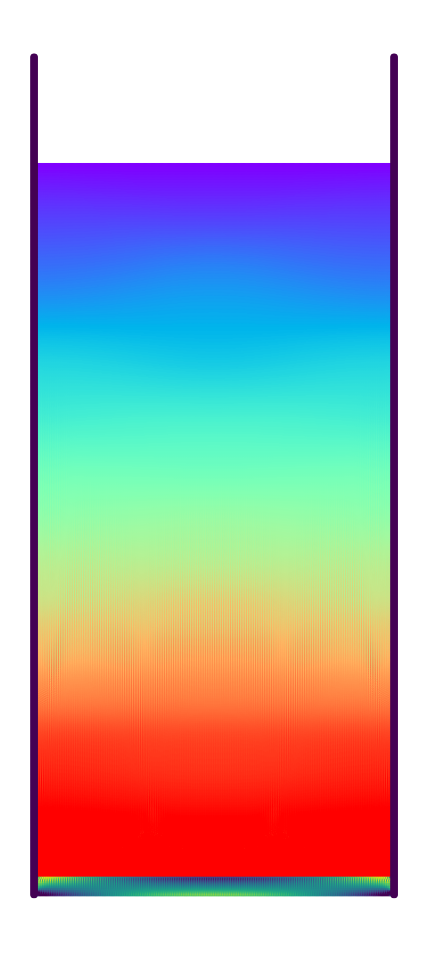
\includegraphics[scale=1.0]{figures/fsi/figures/ng_2020_hydrostatic_water_column_on_elastic_plate/snap_t_0}
  \end{subfigure}
  \begin{subfigure}{0.48\textwidth}
    \centering
    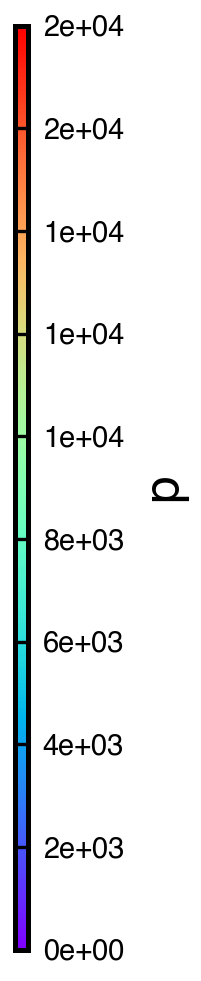
\includegraphics[scale=1.0]{figures/fsi/figures/ng_2020_hydrostatic_water_column_on_elastic_plate/colorbar_t_0}
  \end{subfigure}
  \caption{ Snapshot of the fluid and the elastic structure at time 0.5 sec
   including the pressure of the fluid.}
\label{fig:snapshot-hs-fsi}
\end{figure}
demonstrating the stability of the current solver.
\Cref{fig:ng2020hsplate:deflection} depicts the time history of y-displacement
of the beam center for different particle resolutions computed using the current
solver compared against the analytical solution. From
\cref{fig:ng2020hsplate:deflection} we can see that the current solver is able
to predict the displacement of the clamped beam within the vicinity of the
analytical results. The current solver's beam displacement is closer to the
numerical results provided by \cite{ng2020coupled}. The convergence of the
beam displacement is shown with the particle spacing is reduced.
\begin{figure}
  \centering
  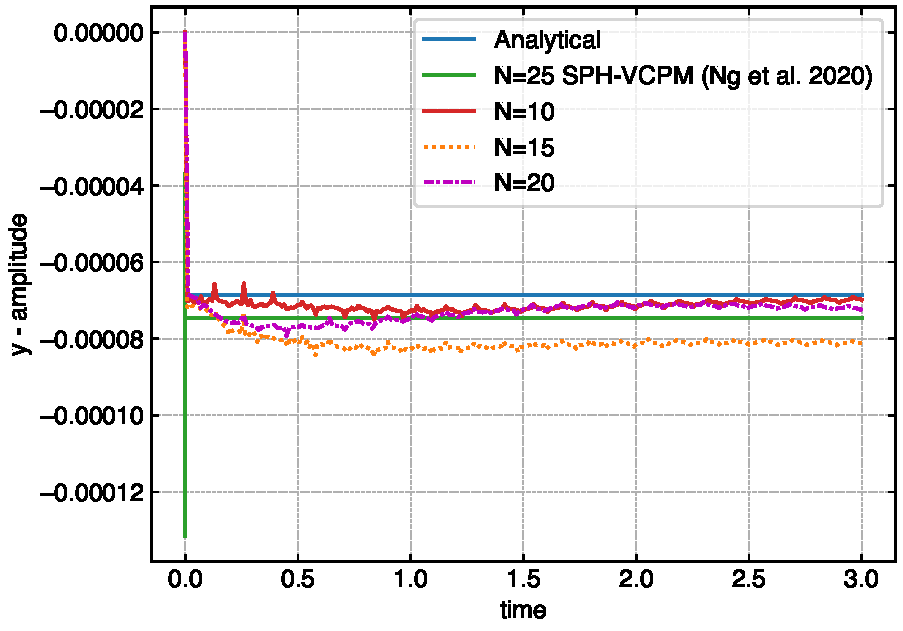
\includegraphics[scale=0.5]{{{figures/fsi/figures/ng_2020_hydrostatic_water_column_on_elastic_plate/y_amplitude}}}
  \caption{The mid-span deflection of the structure under hydrodynamic loading
    with time for different resolutions, compared against the analytical and
    the numerical result of \citep{ng2020coupled}.}
\label{fig:ng2020hsplate:deflection}
\end{figure}
%


\subsection{Water Impact onto an Elastic Plate}
\label{sec:water-impact-forefront}
In this case, we study the deformation of the elastic
plate due to the impact of water from a dam break.
\Cref{fig:dam-break-flow-impact-plate-initial-setup} shows the initial positions
of fluid and the structure inside the dam, including the dimensions. Following
\cite{sun2019fully}, we set the material properties of the elastic plate with a
density of $2500$ kgm\textsuperscript{-3}, Young's modulus of $10^6$ Pa, and a
Poisson ratio of $0$. The material properties of the fluid are a density of 1000
kgm\textsuperscript{-3}, with no dynamic viscosity. A particle spacing of $5$
$\times$ $10^{-4}$ m is taken, resulting in a total of $182911$ particles, which
includes fluid, structure, and solid wall. We simulate a total physical time of
$0.7$ seconds. Here, the fluid is allowed to settle under gravity inside the
tank and attains a velocity as it reaches the elastic structure. The structure
will obstruct the fluid, making it rise, and the fluid will deform the elastic
plate. The rising fluid will hit the other end of the dam, come back, and hit
the structure from the back. We compare the current solver results to the other
numerical techniques for quantitative validation.
\begin{figure}
  \centering
  \includegraphics[scale=0.4]{images/fsi/images/sun_2019_dam_breaking_flow_impacting_an_elastic_plate/schematic}
  \caption{Schematic of the dam-break flow impacting an elastic plate. All dimensions are in meters.}
\label{fig:dam-break-flow-impact-plate-initial-setup}
\end{figure}

\begin{figure}
  \centering
  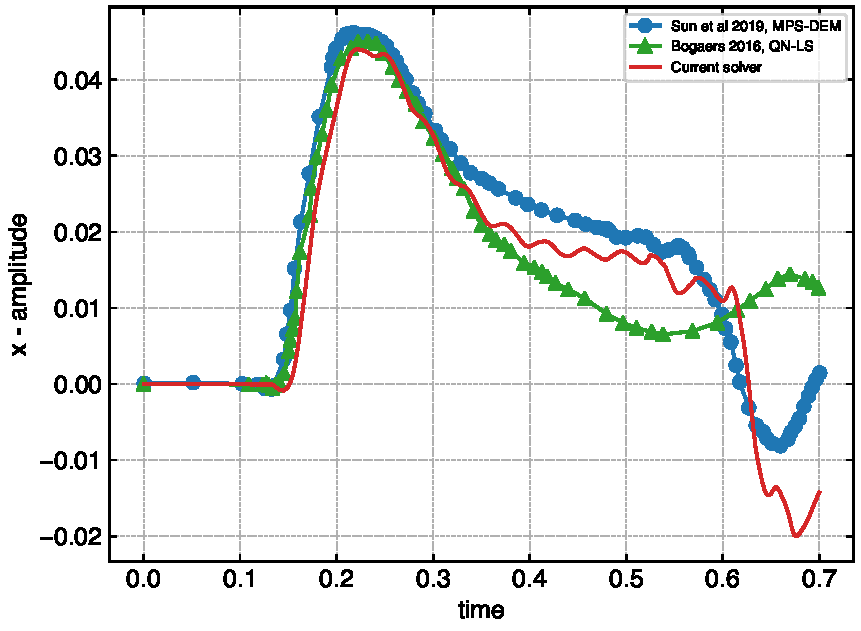
\includegraphics[scale=0.45]{figures/fsi/figures/sun_2019_dam_breaking_flow_impacting_an_elastic_plate/x_amplitude}
  \caption{Time histories of horizontal displacement of the free end of the
    elastic structure compared against the numerical results of
    \citep{sun2019fully,bogaers2016evaluation}- Water impact onto an elastic
    plate.}
\label{fig:water-impact-plate-deflection-quantitative}
\end{figure}
\begin{figure}[H]
    \centering
  \begin{subfigure}{0.48\textwidth}
    \centering
        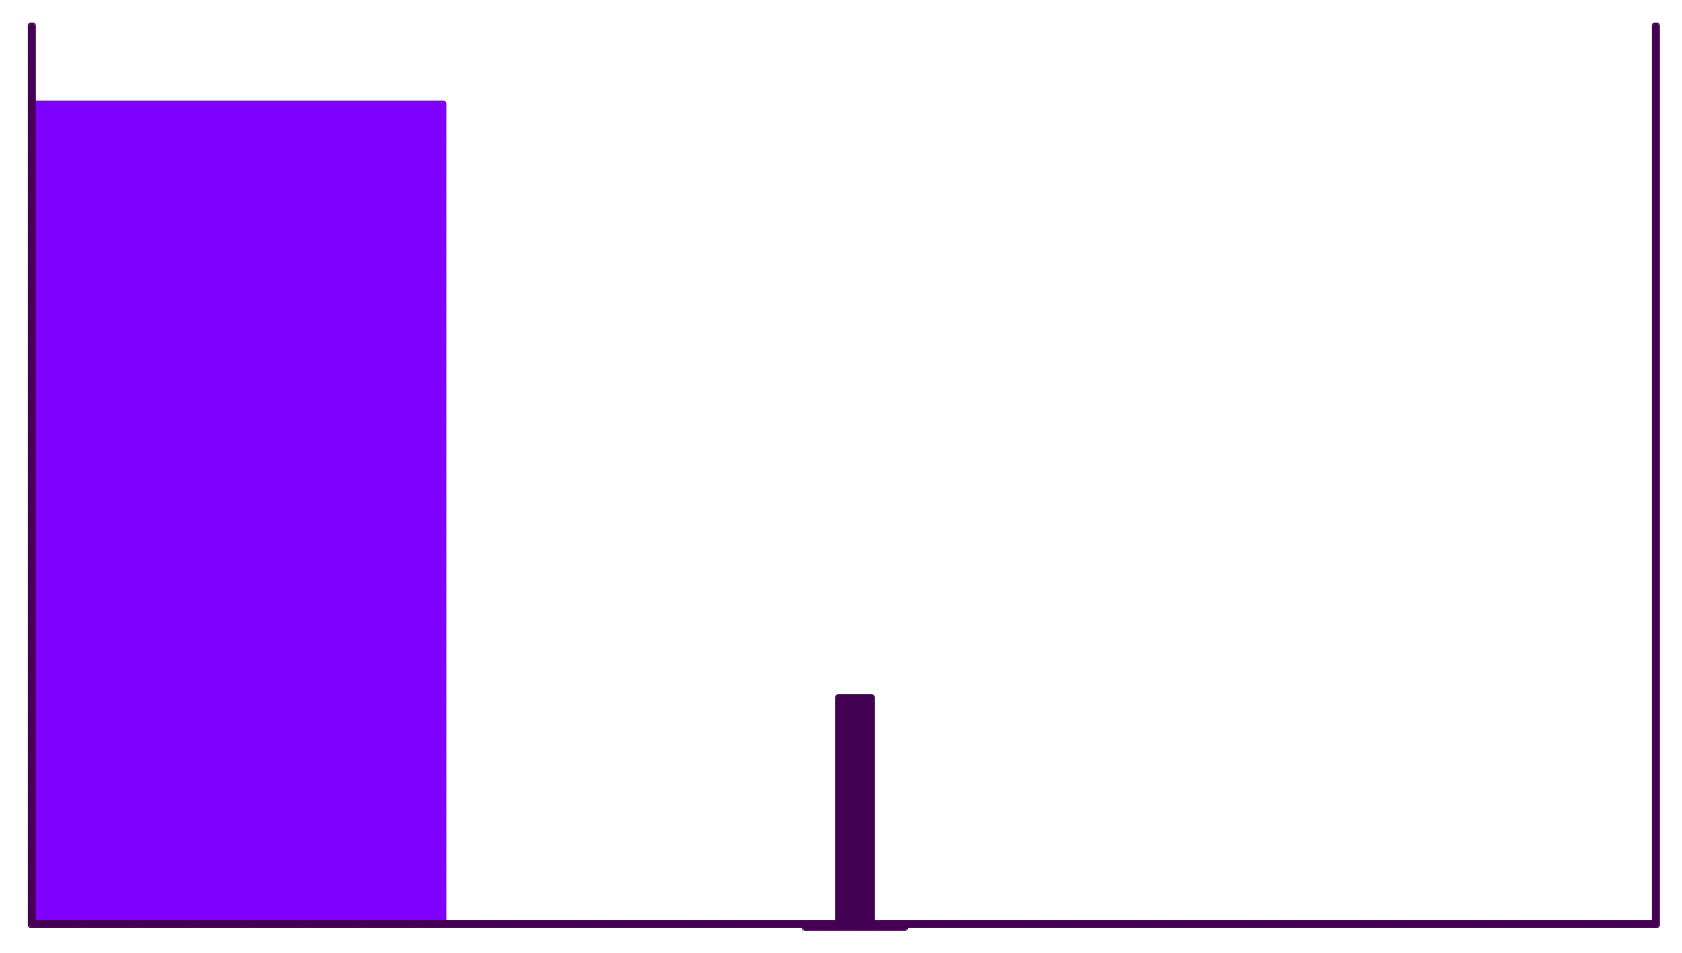
\includegraphics[scale=0.5]{figures/fsi/figures/sun_2019_dam_breaking_flow_impacting_an_elastic_plate/snap_t_0.png}
  \end{subfigure}

  \begin{subfigure}{0.48\textwidth}
    \centering
        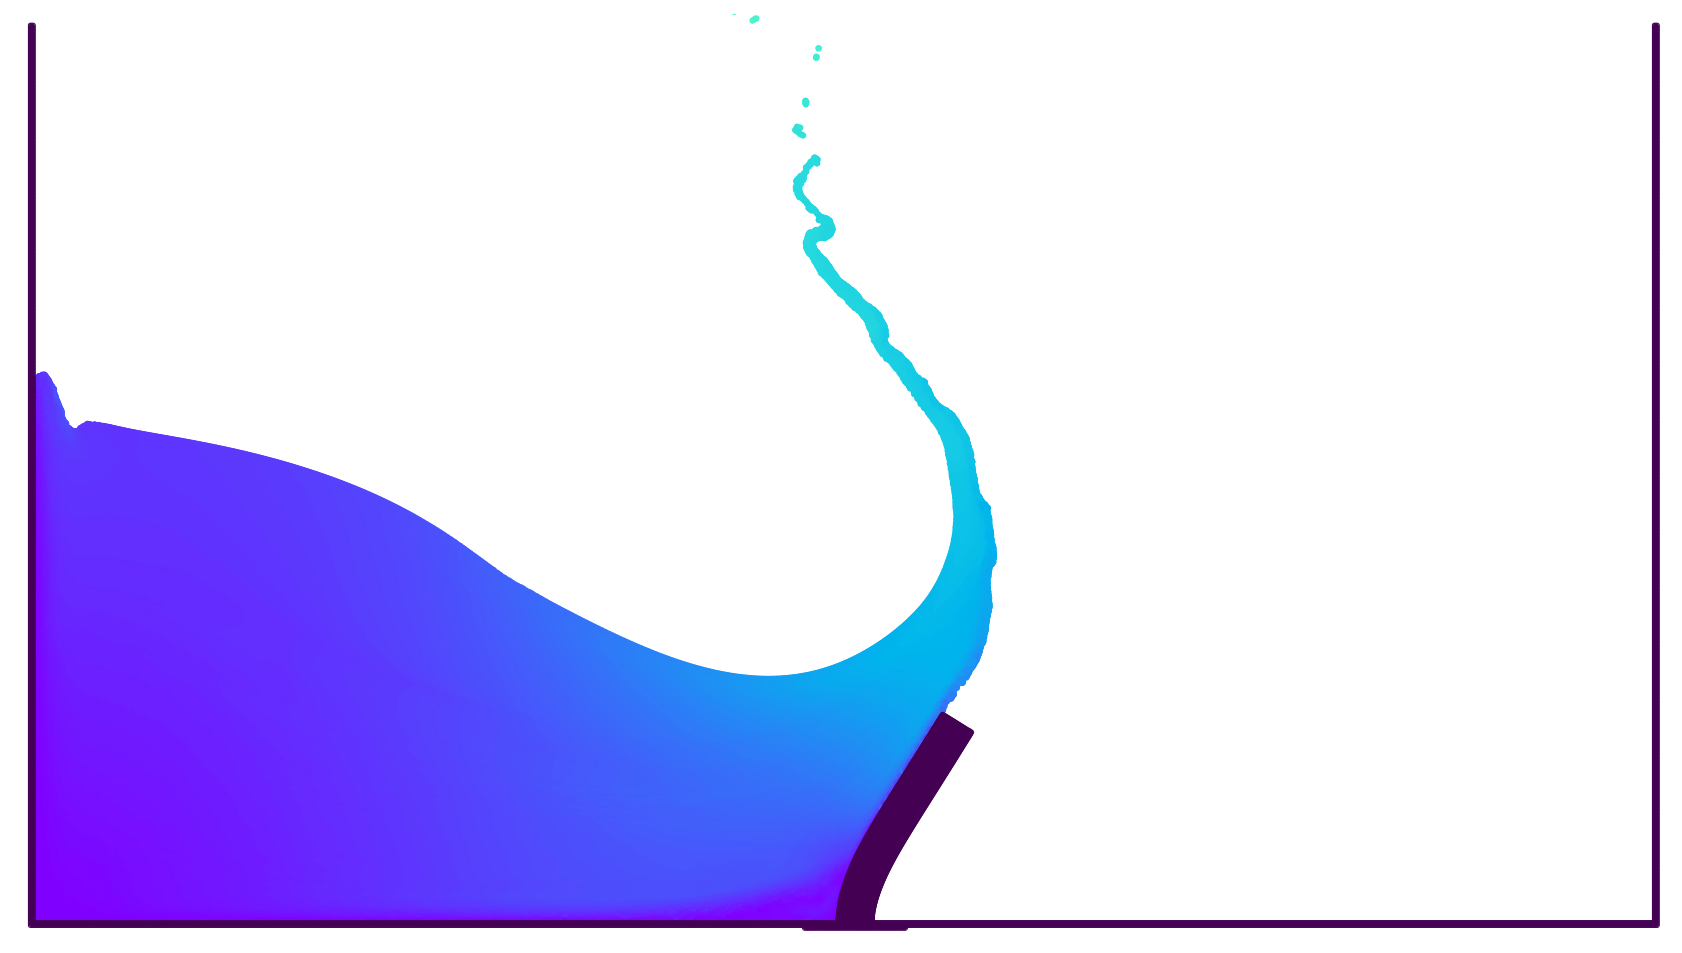
\includegraphics[scale=0.5]{figures/fsi/figures/sun_2019_dam_breaking_flow_impacting_an_elastic_plate/snap_t_1.png}
  \end{subfigure}

  \begin{subfigure}{0.48\textwidth}
    \centering
        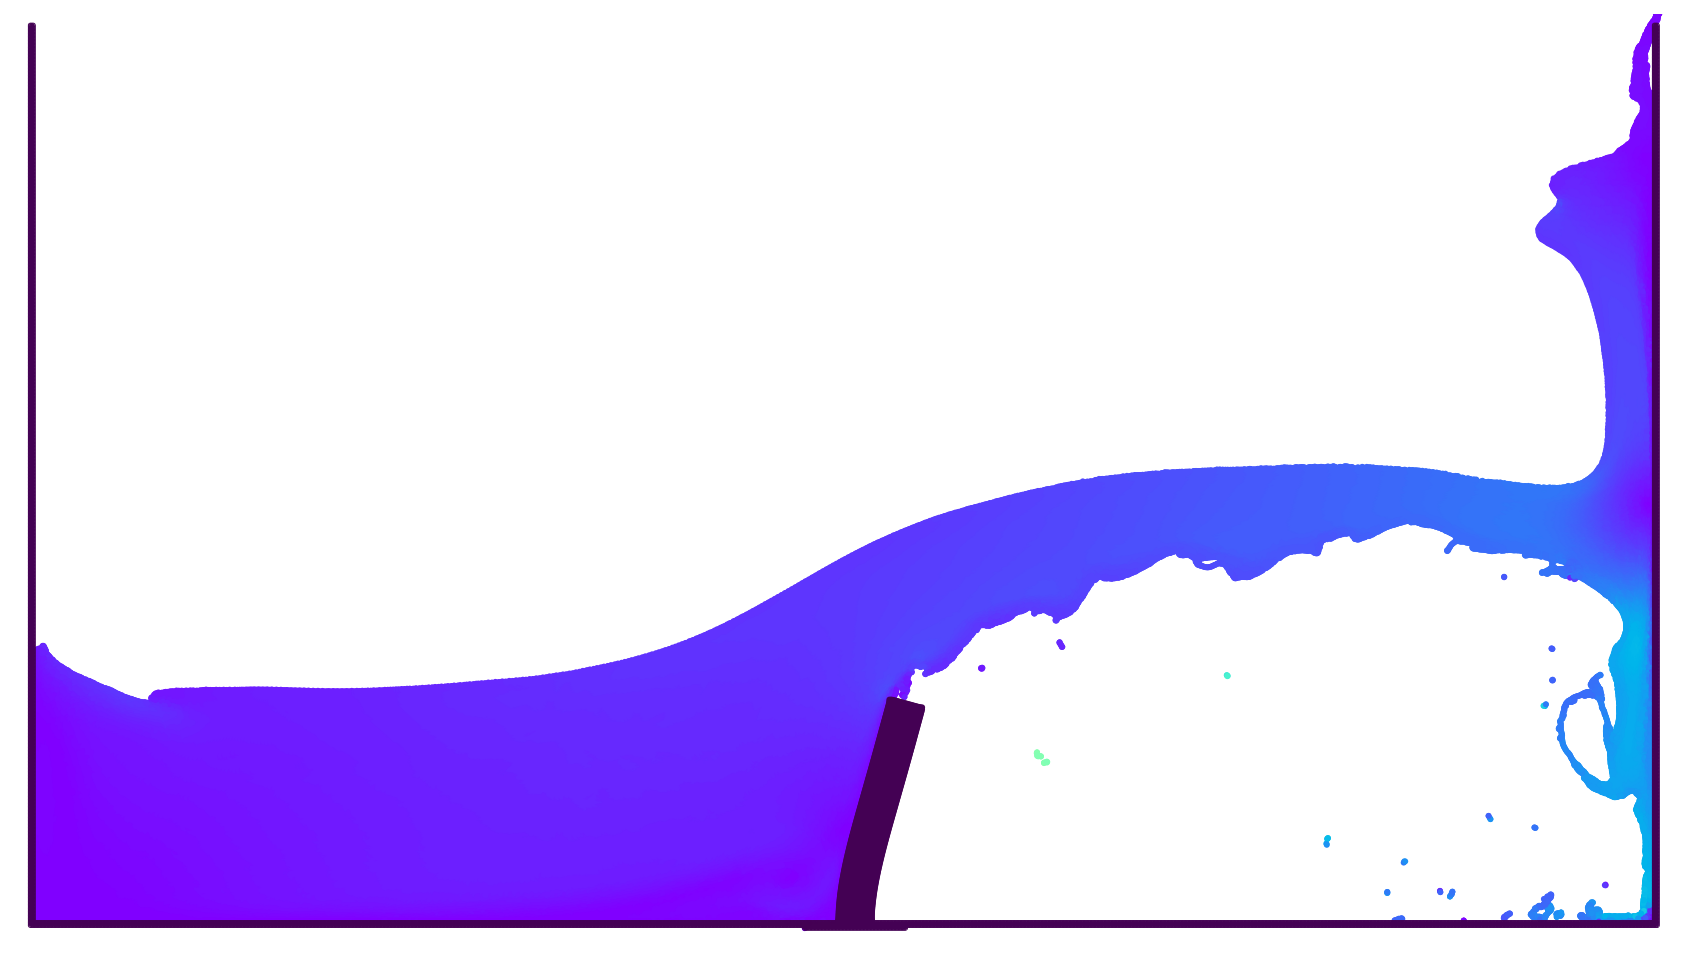
\includegraphics[scale=0.5]{figures/fsi/figures/sun_2019_dam_breaking_flow_impacting_an_elastic_plate/snap_t_2.png}
  \end{subfigure}

  \begin{subfigure}{0.48\textwidth}
    \centering
        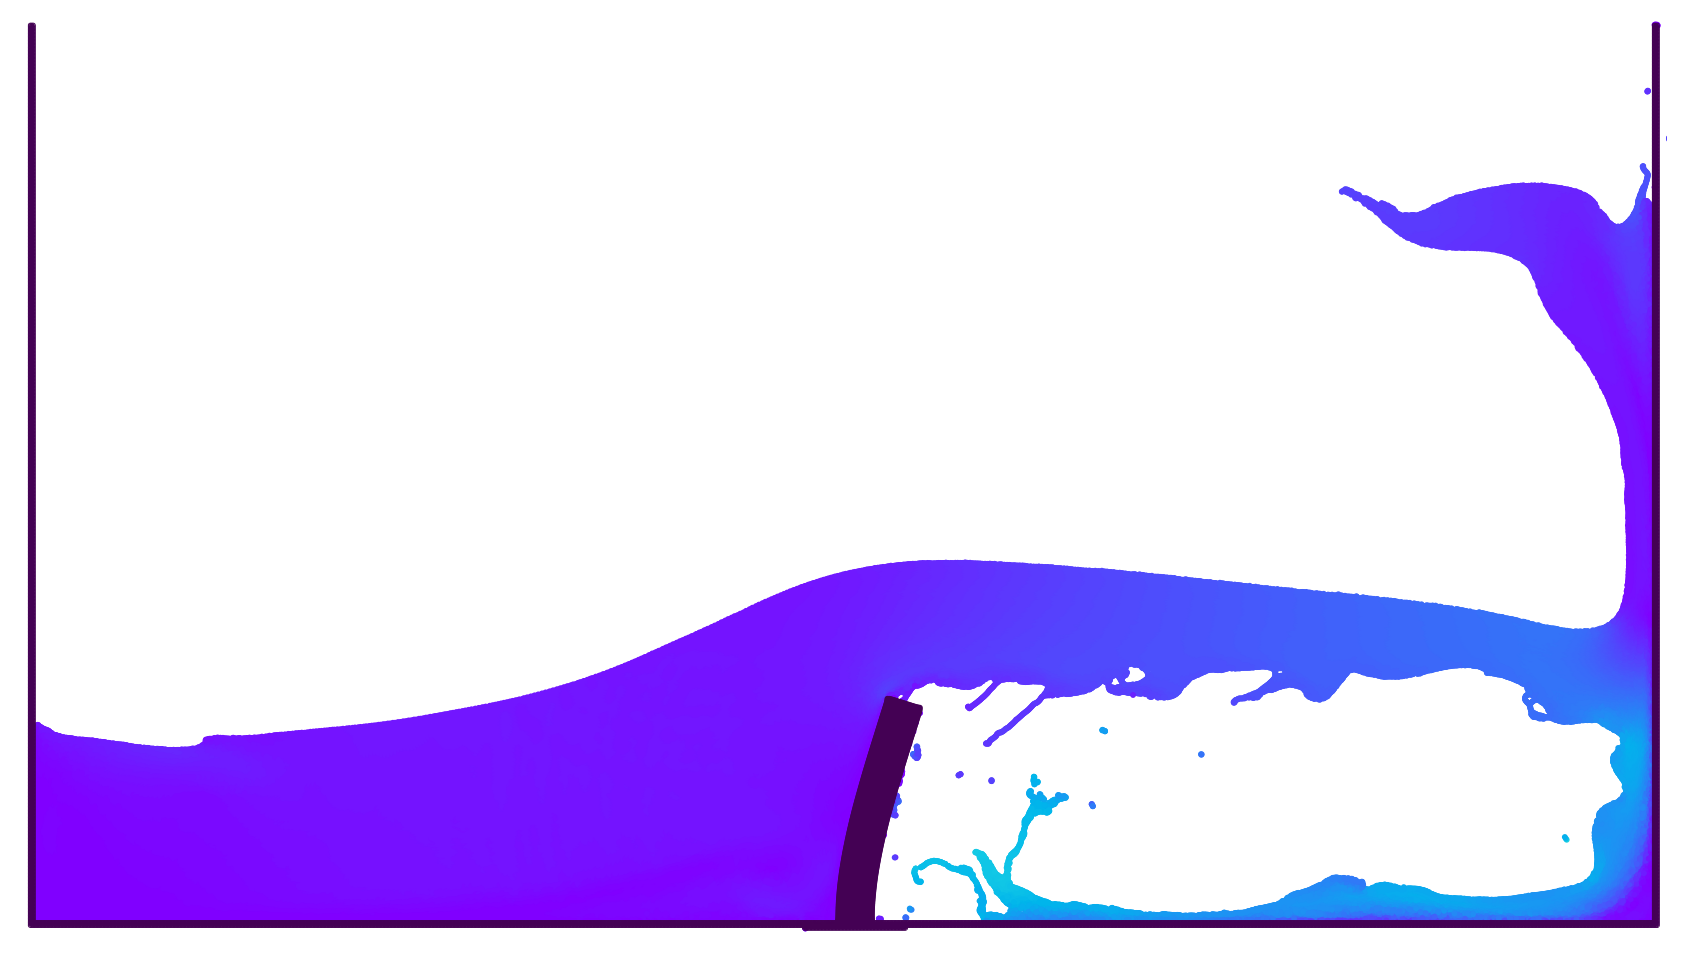
\includegraphics[scale=0.5]{figures/fsi/figures/sun_2019_dam_breaking_flow_impacting_an_elastic_plate/snap_t_3.png}
  \end{subfigure}

  \begin{subfigure}{0.48\textwidth}
    \centering
    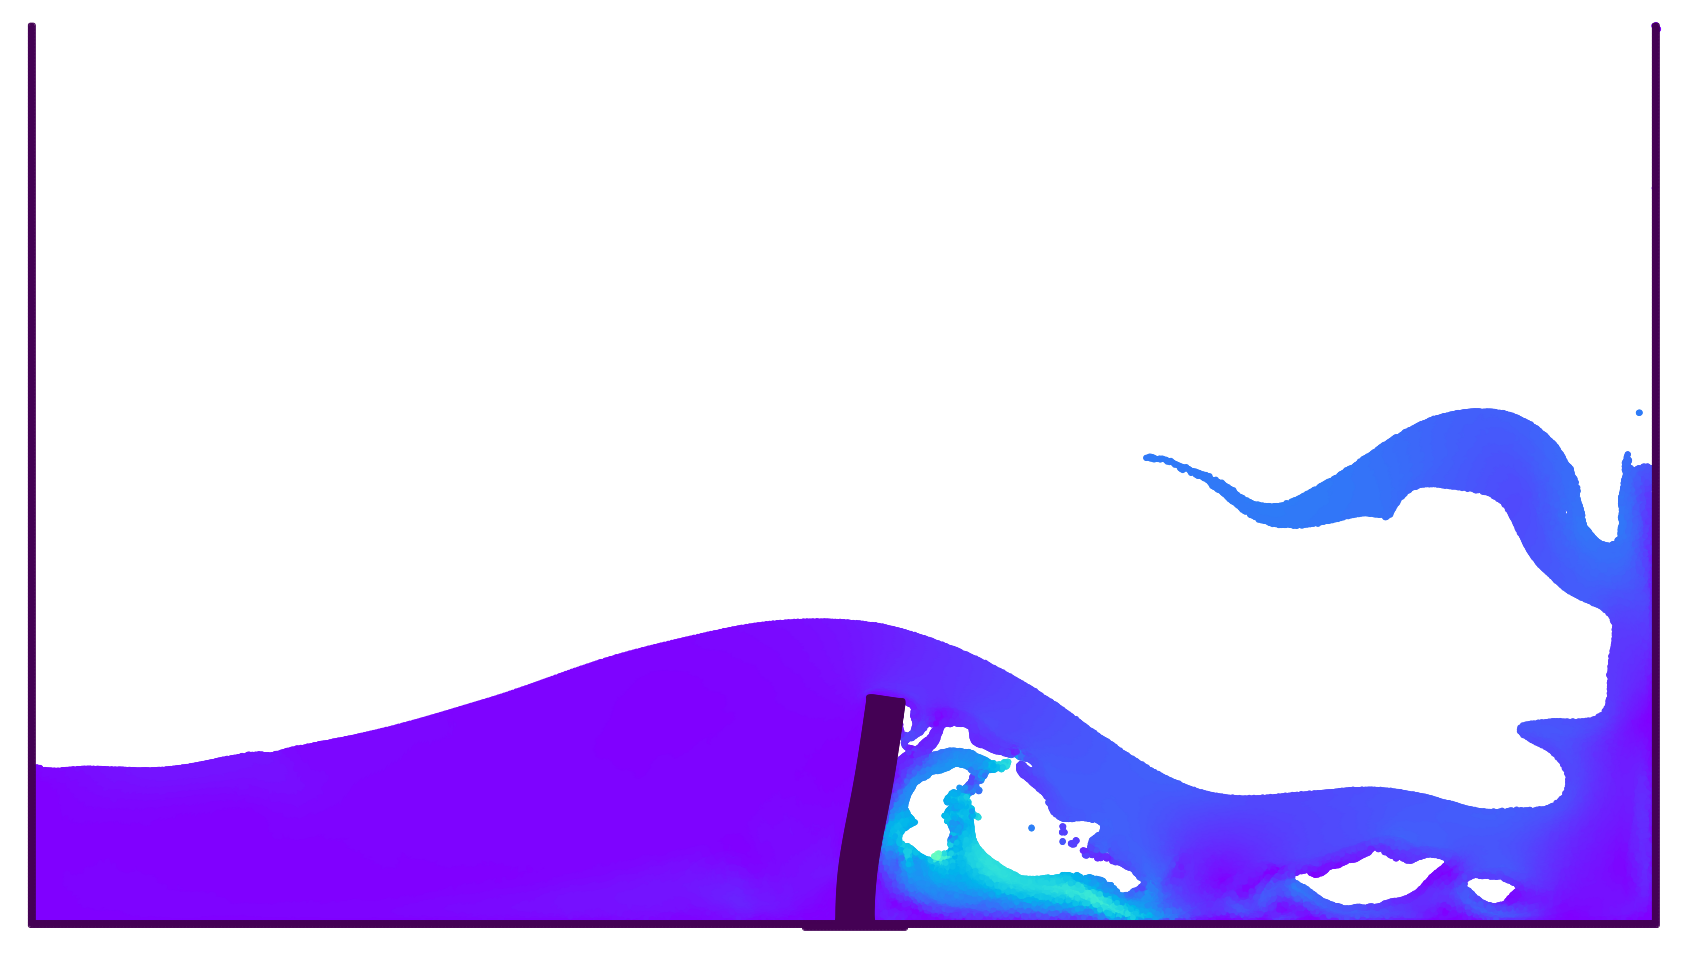
\includegraphics[scale=0.5]{figures/fsi/figures/sun_2019_dam_breaking_flow_impacting_an_elastic_plate/snap_t_4.png}
  \end{subfigure}
    \caption
    {
        Snapshot of the fluid and the structure at different time stamps.
    }
    \label{fig:dam-breaking-onto-plate-snapshot}
\end{figure}
The time variation of the x-displacement of the elastic structure is compared
against other numerical results~\citep{sun2019fully,bogaers2016evaluation}. From
the \cref{fig:water-impact-plate-deflection-quantitative}, we can see that the
displacement computed by the current solver is within the vicinity of the other
results produced. \Cref{fig:dam-breaking-onto-plate-snapshot} shows the
snapshots of the fluid and the elastic structure at different time instances.
From \cref{fig:dam-breaking-onto-plate-snapshot}, we can see that the fluid,
after hitting the structure, rises and hits the other end of the tank and
travels back to hit the structure again.

% ========================================================
% ========================================================
\section{Summary}\label{fsi:summary}
% ========================================================
% ========================================================
In the current chapter, we have handled the fluid-structure interaction using
the CTVF scheme developed in \cref{chap:ctvf}. Through particle shifting
techniques and incorporating the missing terms, we are able to eliminate several
issues SPH faces while solving fluid and solid problems. CTVF improves the
accuracy of fluid problems, and eliminates tensile instability while solving
elastic dynamics problems without any additional artificial stress terms.

We validated the developed scheme by solving a UDL problem to test the structure
equations, and an aluminum plate over a hydrostatic tank where an analytical
solution is available is utilized to validate the FSI part of the current
solver. The current solver is applied to a dam break hitting an elastic plate.
Here, the deformation of the elastic plate is compared to the computational
results of other numerical models. A convergence analysis is undertaken for both fundamental benchmarks,
UDL, and hydrostatic tank.

FSI is one essential multiphysics problem to be modeled in order to simulate
complex physical processes. In the next chapter we will consider the rigid-fluid
coupling as it allows us to study coupled behaviour of fluid and rigid body
together.
